\documentclass[slidestop,usenames,dvipsnames]{beamer}
\usepackage[utf8]{inputenc}
\usepackage[T1]{fontenc}
\usepackage[absolute,overlay]{textpos}
\usepackage{graphicx}
\usepackage[yyyymmdd]{datetime}
\renewcommand{\dateseparator}{-}

\title{Watts' Network Cascades Model}
\subtitle{A Simple Model of Global Cascades on Random Networks}
\author{Marco Brack \and Carsten Hartenfels}

\beamertemplatenavigationsymbolsempty
\usetheme{Boadilla}
\usecolortheme{whale}
\setbeamertemplate{itemize items}[default]
\setbeamertemplate{enumerate items}[default]
\defbeamertemplate*{footline}{my infolines theme} {
    \leavevmode
    \hbox{
    \begin{beamercolorbox}[wd=.333333\paperwidth,ht=2.25ex,dp=1ex,center]{author in head/foot}
        \usebeamerfont{author in head/foot}Marco Brack, Carsten Hartenfels
    \end{beamercolorbox}
    \begin{beamercolorbox}[wd=.333333\paperwidth,ht=2.25ex,dp=1ex,center]{title in head/foot}
        \usebeamerfont{title in head/foot}Watts' Network Cascades Model
    \end{beamercolorbox}
    \begin{beamercolorbox}[wd=.309\paperwidth,ht=2.25ex,dp=1ex,center]{date in head/foot}
        \usebeamerfont{date in head/foot}\insertshortdate{}\hspace*{2em}
        \insertframenumber{} / \inserttotalframenumber\hspace*{2ex}
    \end{beamercolorbox}}
    \vskip0pt
}

\newcommand{\fitem}{\pause\vfill\item}
\newcommand{\gitem}{\vfill\item}

\begin{document}

\begin{frame}
    \titlepage
\end{frame}


%%%%%%%%%%%%%%%%%%%%%%%%%%%%%%%%%%%%%%%%%%%%%%%%


\begin{frame}
    \frametitle{Content}
    \begin{itemize}
        \gitem Motivation
        \gitem Simulation
        \gitem Explanation
        \gitem Watts' Model
        \gitem Findings
        \gitem Limitations
    \end{itemize}
    \vfill
\end{frame}


\begin{frame}
    \frametitle{Motivation -- Culture}
    \begin{center}
        
\includegraphics[height=0.65\textheight]{img/twilight}
        \vfill\vspace{8pt}
        {\huge Twilight}
        \vfill\vspace{8pt}
        {\small Source: \url{https://en.wikipedia.org/wiki/File:Twilightbook.jpg}}
    \end{center}
    \vfill
\end{frame}

\begin{frame}
    \frametitle{Motivation -- Technology Adoption}
    \begin{center}
        
\includegraphics[height=0.65\textheight]{img/whatsapp}
        \vfill\vspace{8pt}
        {\huge WhatsApp}
        \vfill\vspace{8pt}
        {\small Source: \url{https://commons.wikimedia.org/wiki/File:WhatsApp.svg}}
    \end{center}
    \vfill
\end{frame}

\begin{frame}
    \frametitle{Motivation -- Social Dynamics}
    \begin{center}
        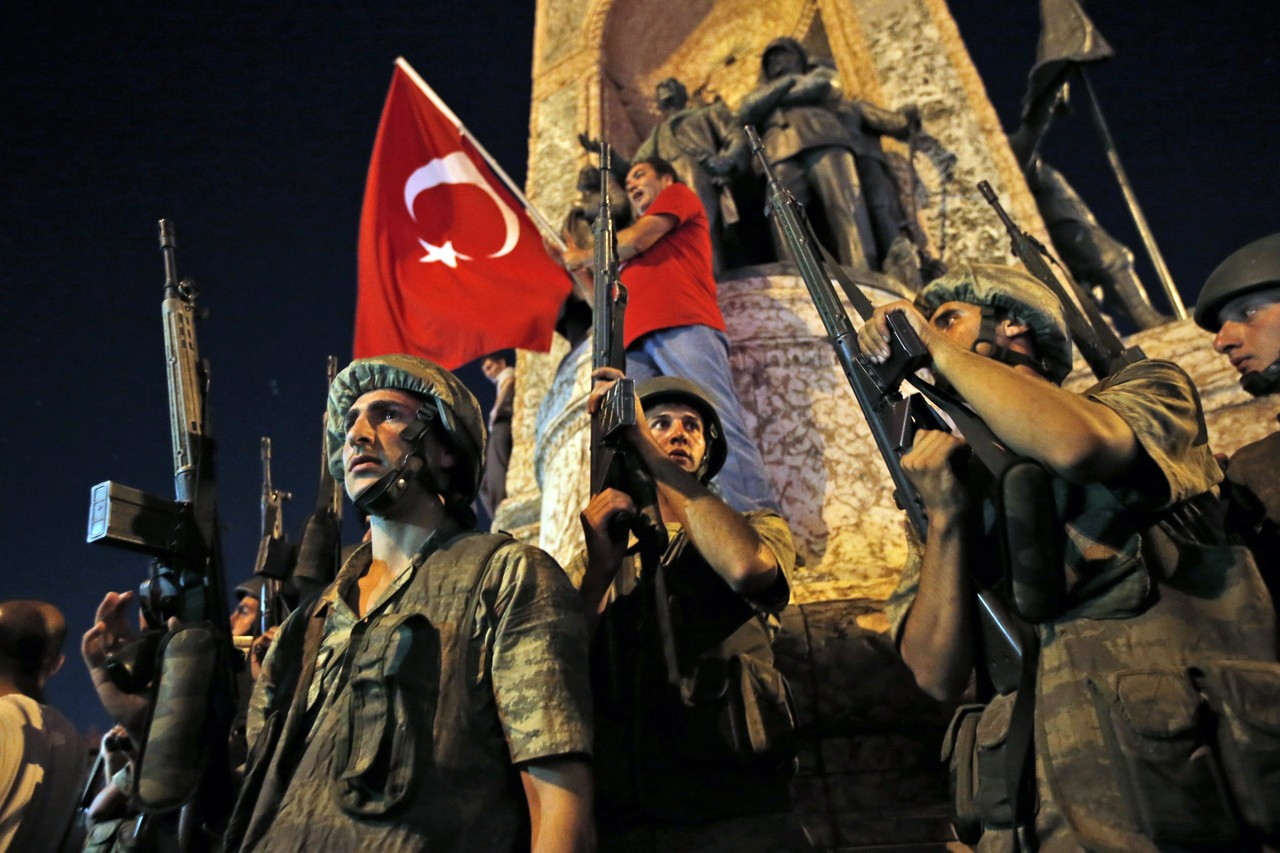
\includegraphics[height=0.65\textheight]{img/coup}
        \vfill\vspace{8pt}
        {\huge Political Coups}
        \vfill\vspace{8pt}
        {\small Source: \url{http://tinyurl.com/jmv529r}}
    \end{center}
    \vfill
\end{frame}

\begin{frame}
    \frametitle{The Cause Revealed}
    \vfill
    \begin{center}
        \pause {\Huge \underline{Network Cascades}}\\
        \vspace{20pt}
        \pause {\footnotesize (Maybe)}\\
        \vspace{20pt}
        \pause {\footnotesize (It's a Nice Model Anyway)}
    \end{center}
    \vfill
\end{frame}

\begin{frame}
    \vfill
    \begin{center}
        {\Huge Simulation}\
        \vfill
        \url{https://github.com/turbopope/nss/tree/master/simulator}
    \end{center}
\end{frame}

% too much clutter
\begin{frame}
    \frametitle{Model of Doom}
    \begin{itemize}
        \gitem Nodes
    \end{itemize}
    \vspace{10.8pt}
    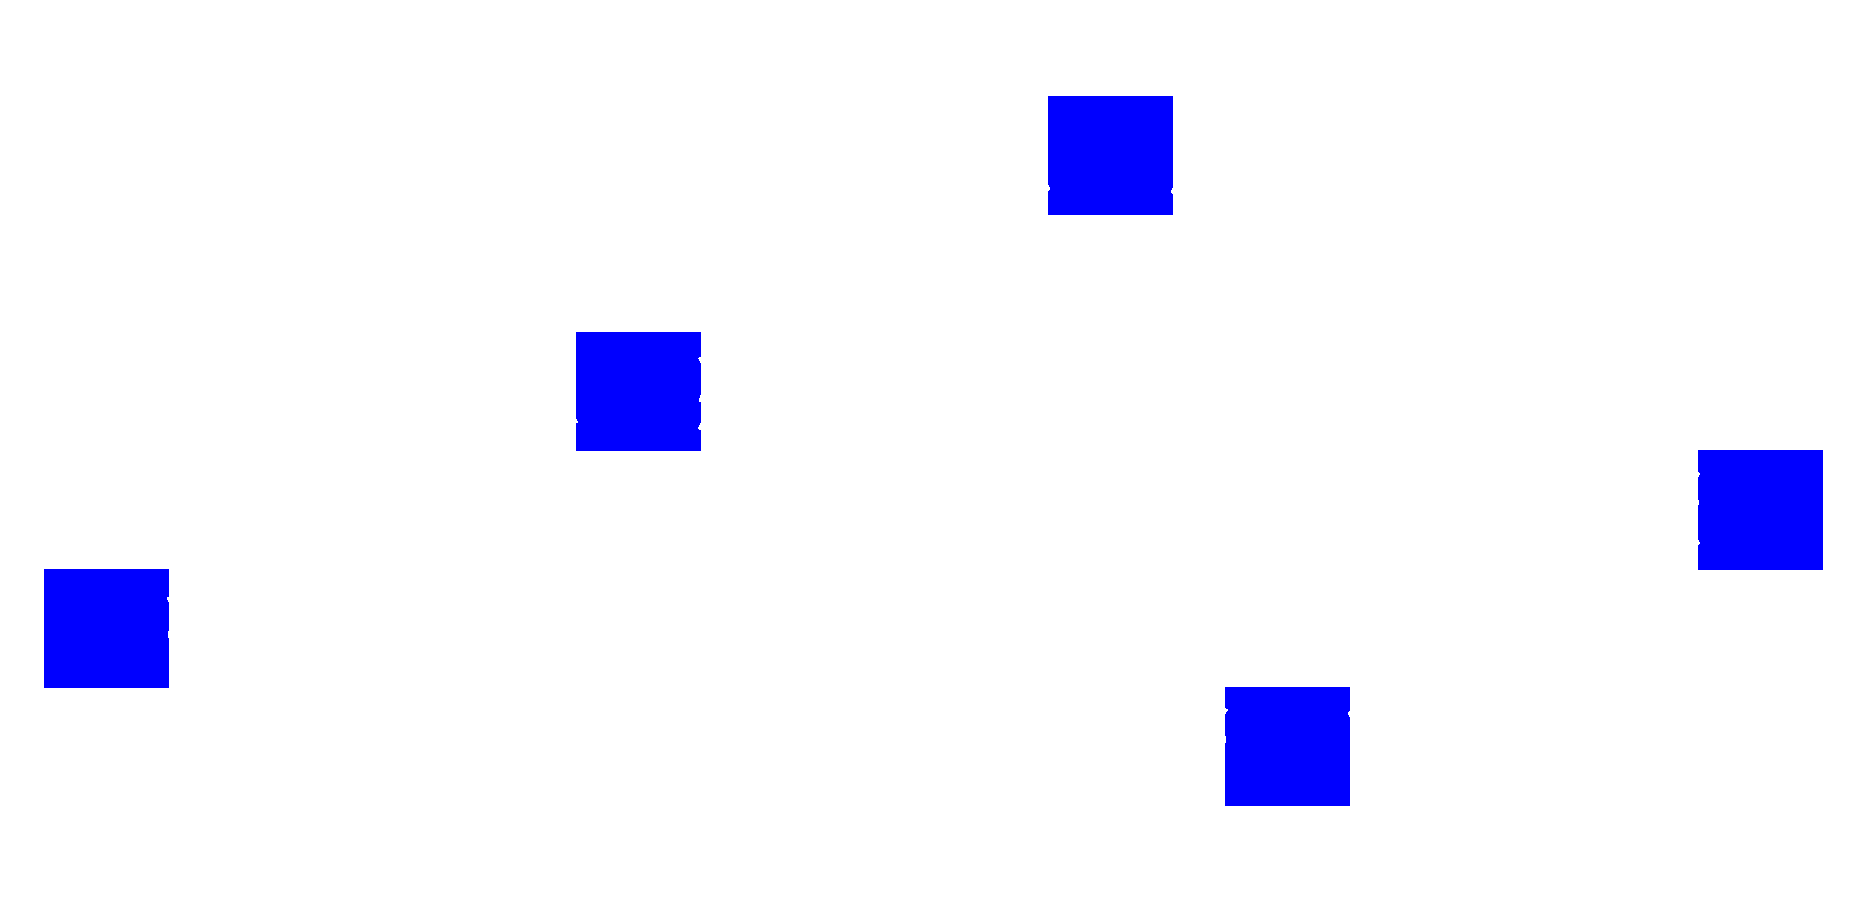
\includegraphics[width=\textwidth]{img/model1}
    \vfill
\end{frame}

\begin{frame}
    \frametitle{Model of Doom}
    \begin{itemize}
        \gitem Observe $k$ Neighbors
    \end{itemize}
    \vspace{8.6pt}
    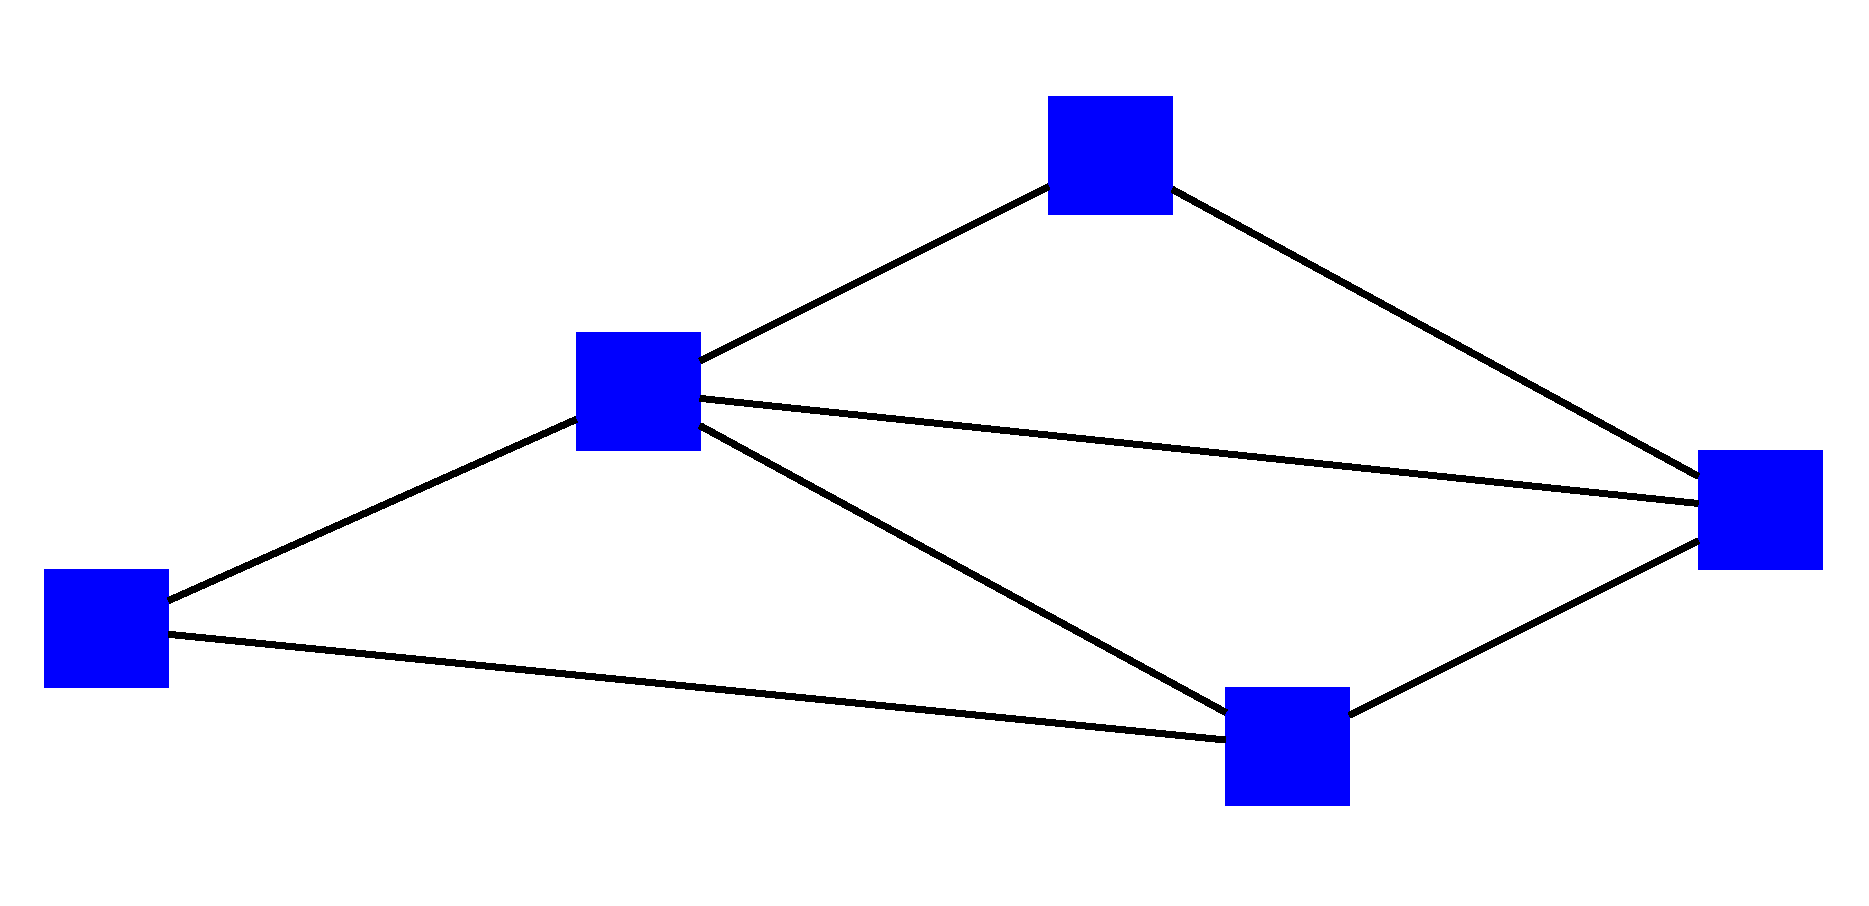
\includegraphics[width=\textwidth]{img/model2}
    \vfill
\end{frame}

\begin{frame}
    \frametitle{Model of Doom}
    \begin{itemize}
        \gitem State $\in \lbrace 0, 1 \rbrace$
    \end{itemize}
    \vspace{8pt}
    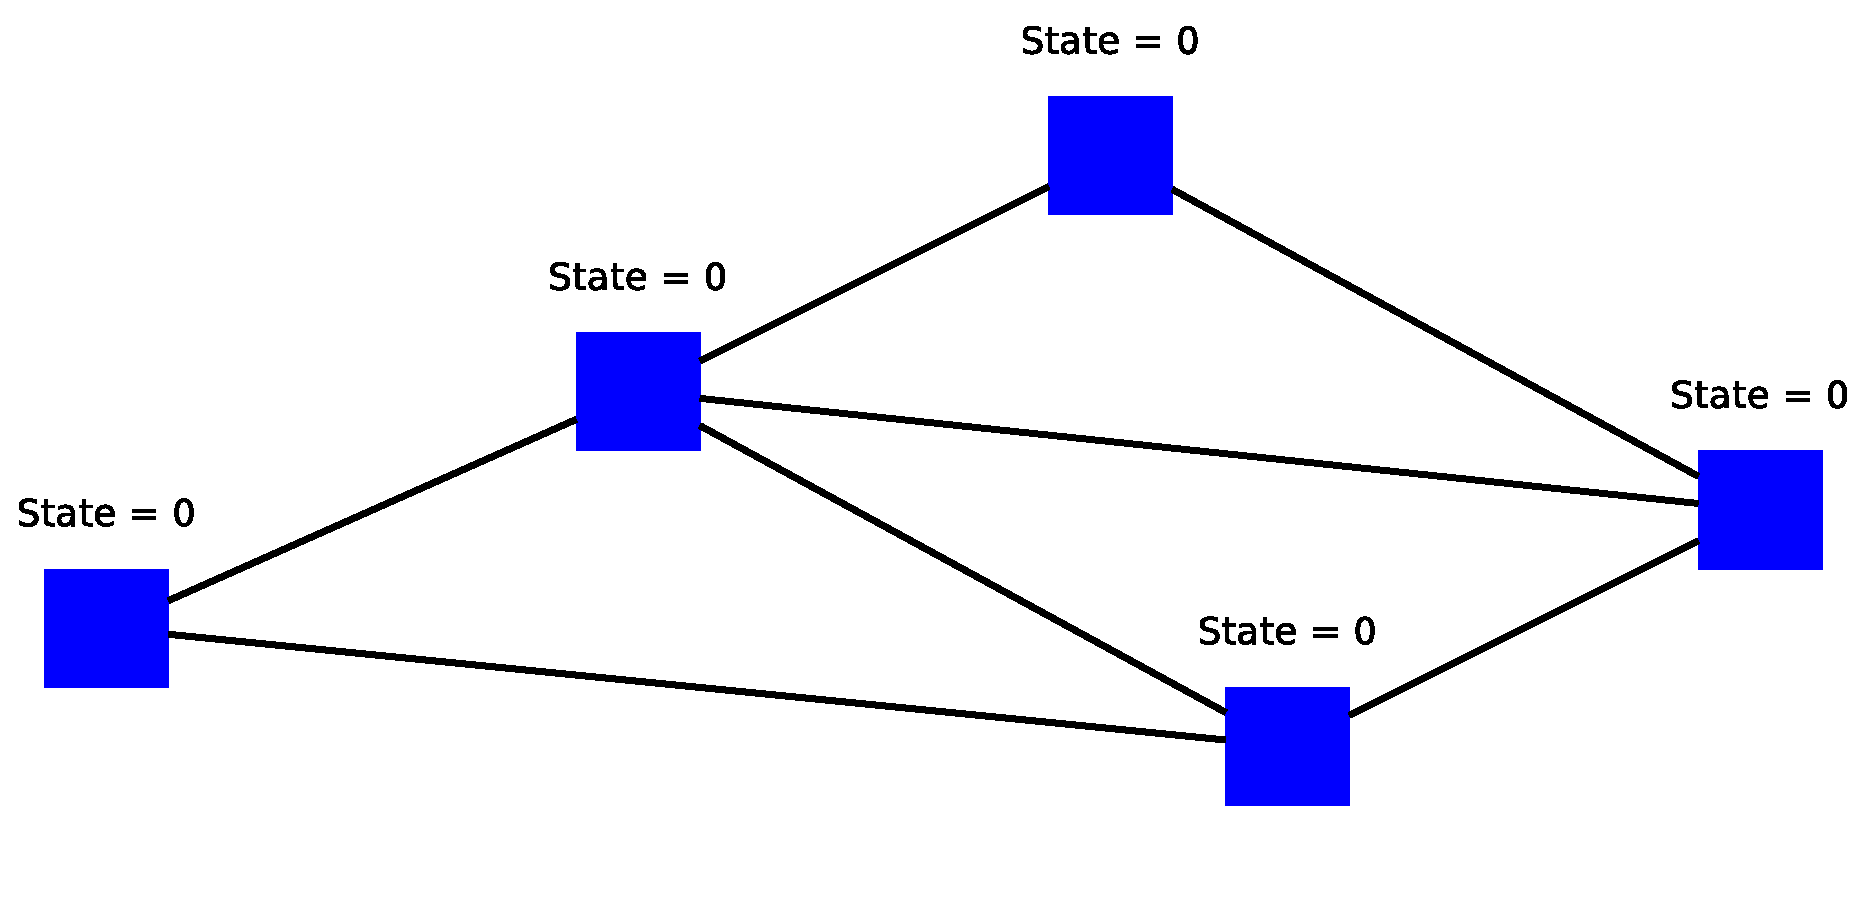
\includegraphics[width=\textwidth]{img/model3}
    \vfill
\end{frame}

\begin{frame}
    \frametitle{Model of Doom}
    \begin{itemize}
        \gitem Threshold $\Phi \in [0, 1]$
    \end{itemize}
    \vspace{8pt}
    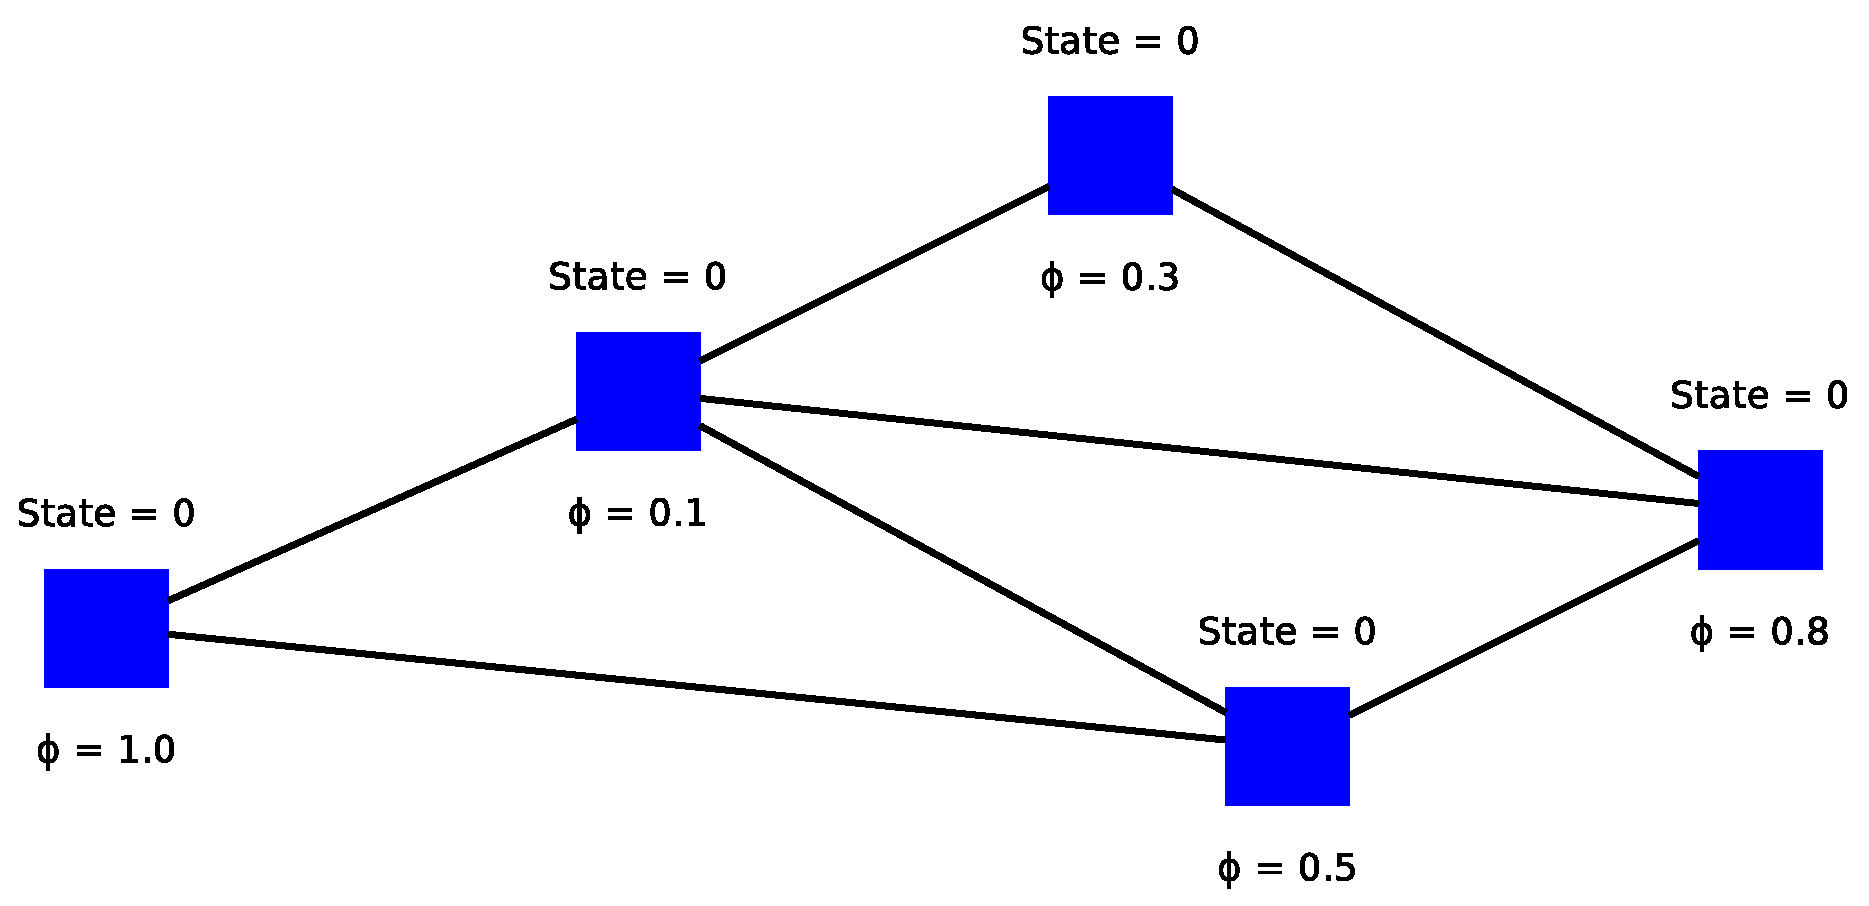
\includegraphics[width=\textwidth]{img/model4}
    \vfill
\end{frame}

\begin{frame}
    \frametitle{Model of Doom}
    \begin{itemize}
        \gitem Random Impulse Happens
    \end{itemize}
    \vspace{8.6pt}
    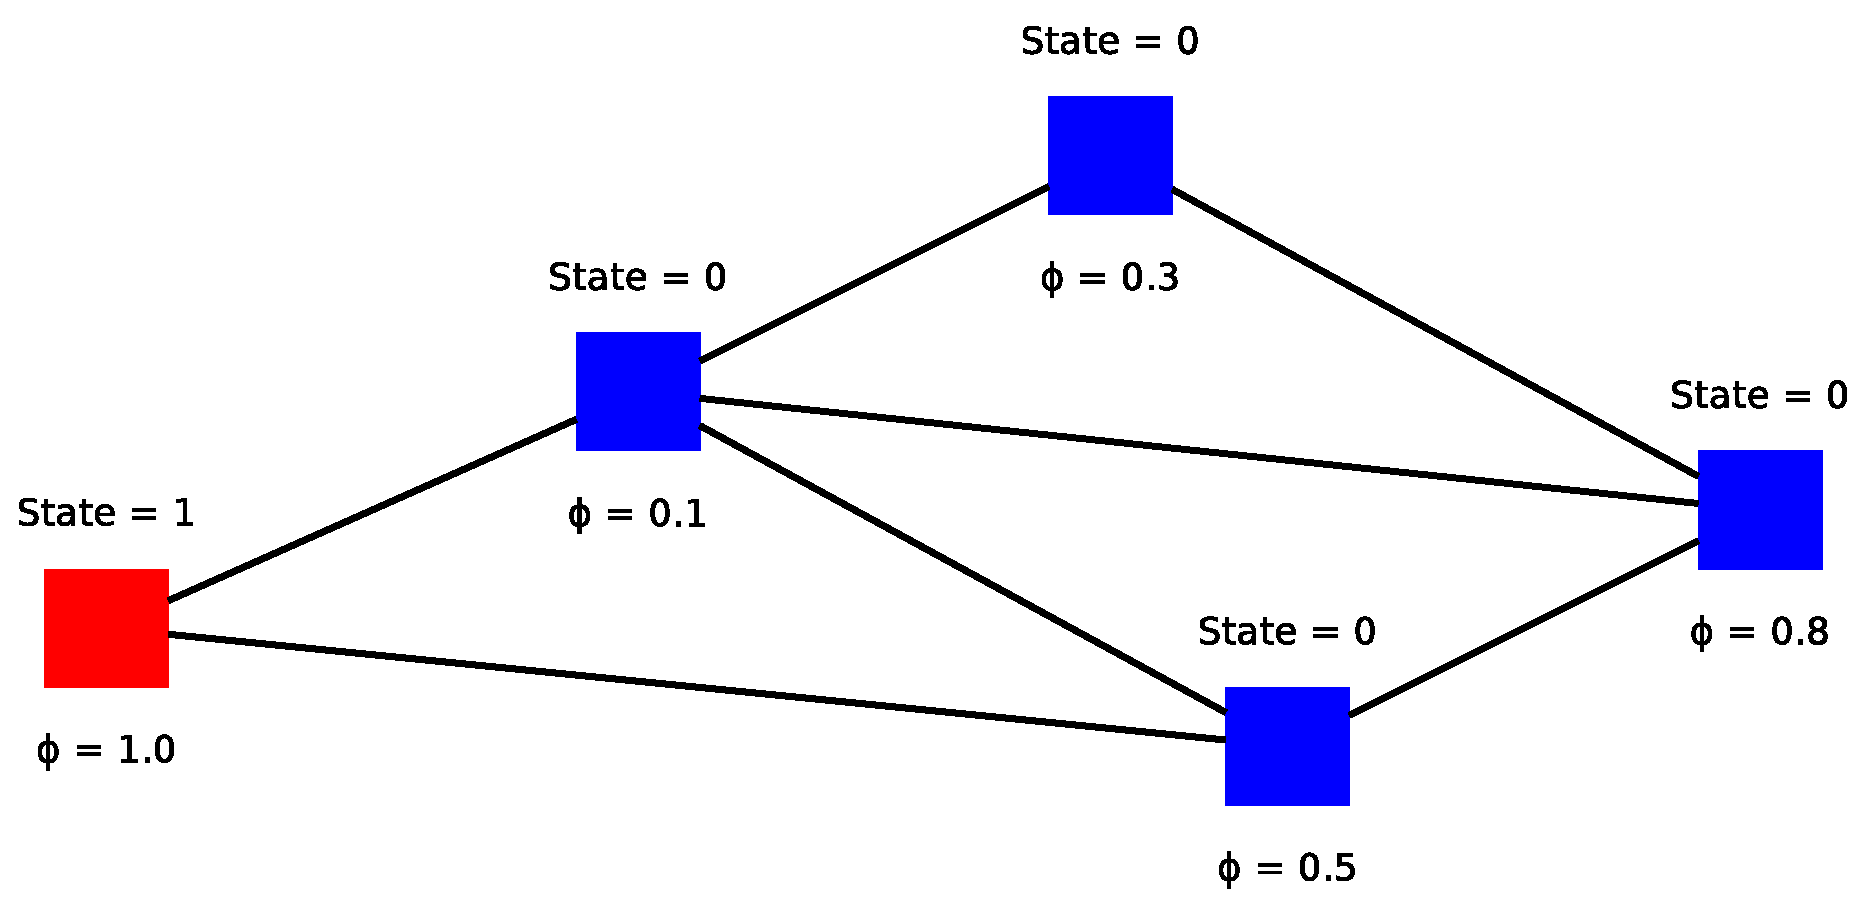
\includegraphics[width=\textwidth]{img/model5}
    \vfill
\end{frame}

\begin{frame}
    \frametitle{Model of Doom}
    \begin{itemize}
        \gitem Nodes Check in Random Intervals
    \end{itemize}
    \vspace{10.8pt}
    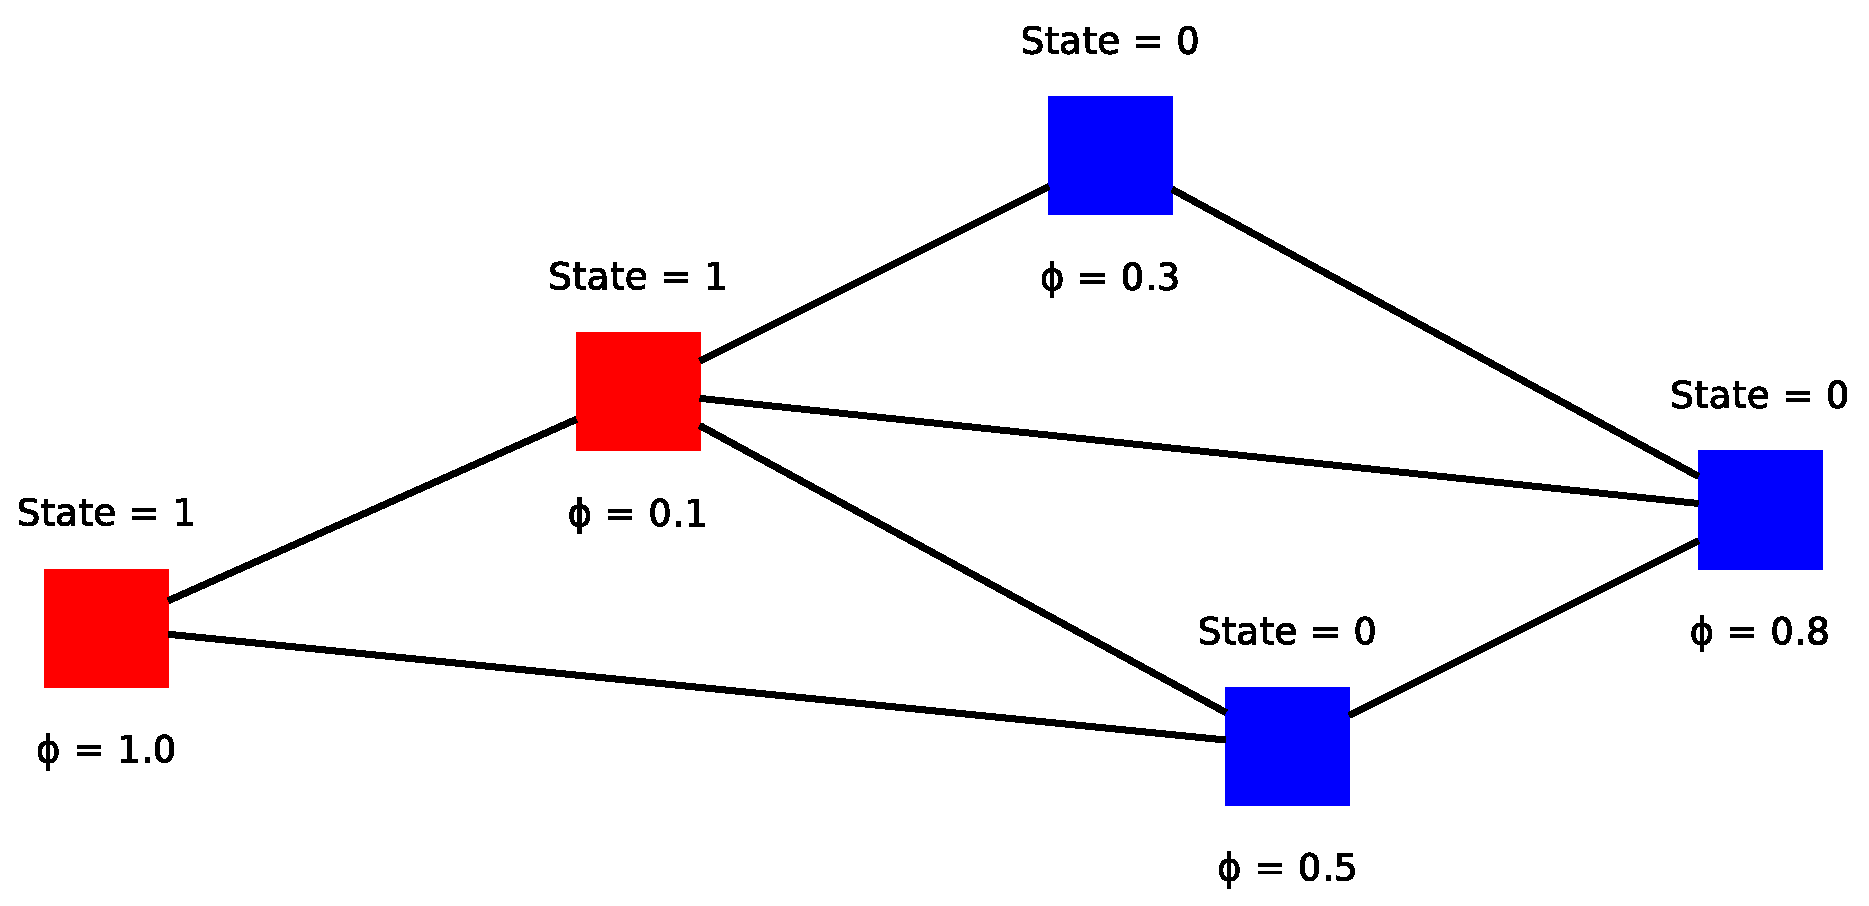
\includegraphics[width=\textwidth]{img/model6}
    \vfill
\end{frame}

\begin{frame}
    \frametitle{Model of Doom}
    \begin{itemize}
        \gitem Stuff Happens
    \end{itemize}
    \vspace{8.8pt}
    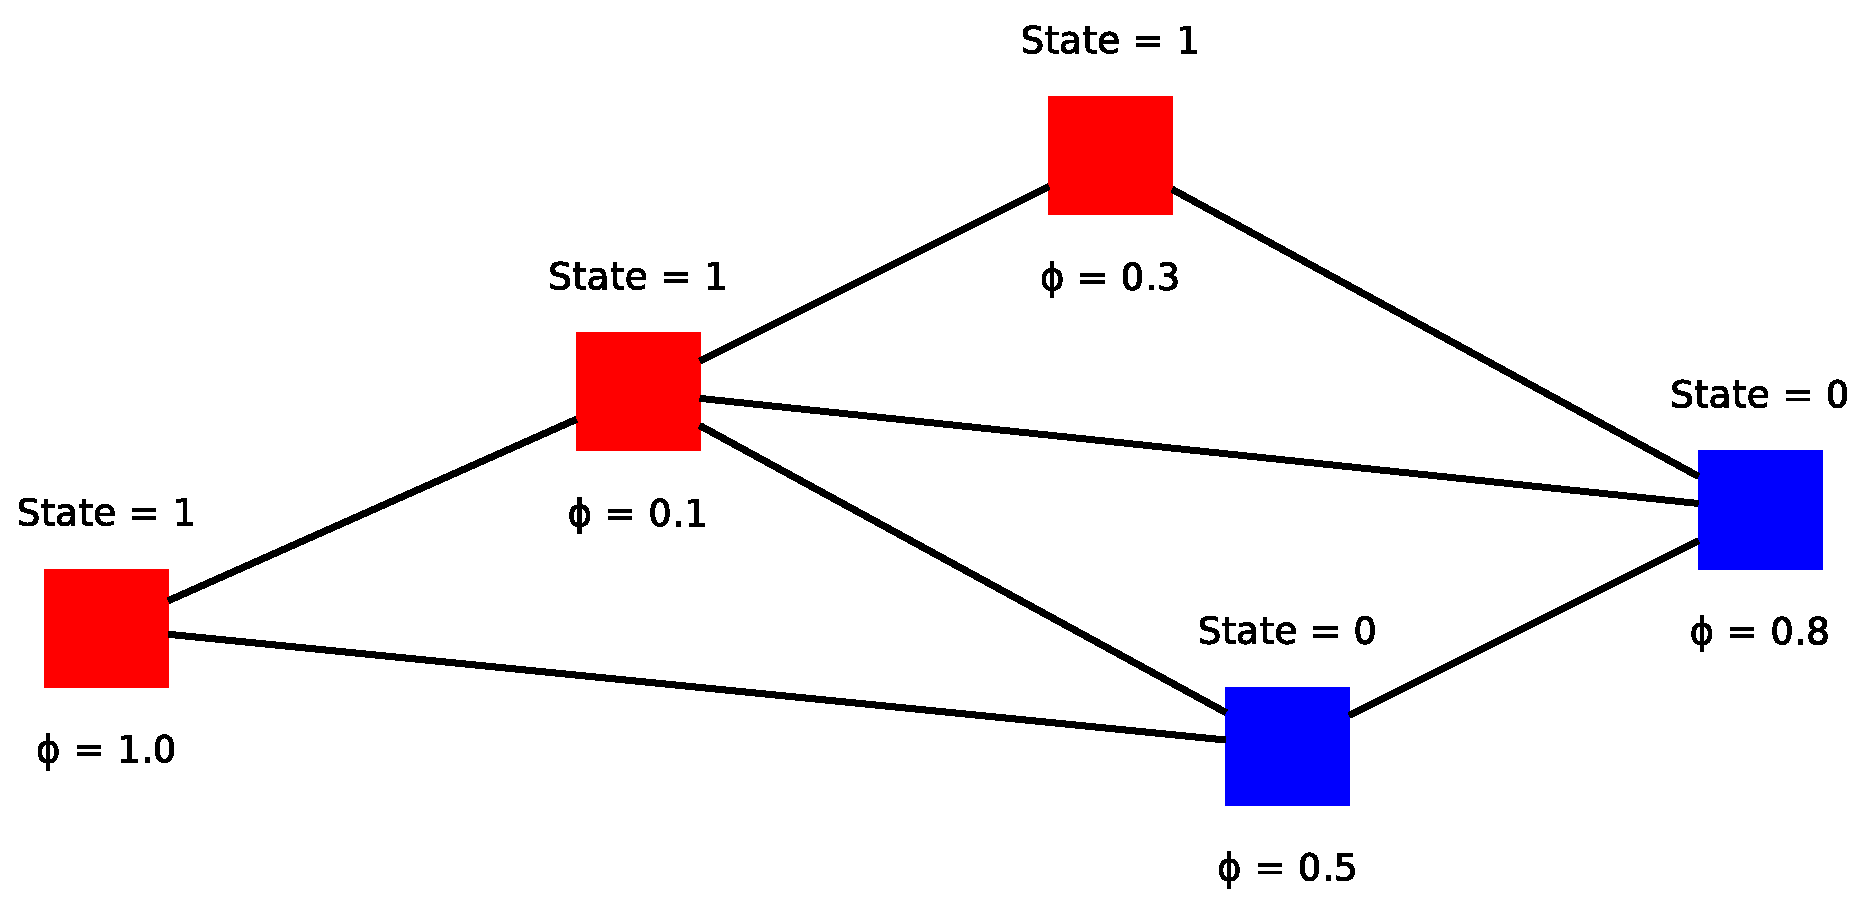
\includegraphics[width=\textwidth]{img/model7}
    \vfill
\end{frame}

\begin{frame}
    \frametitle{Model of Doom}
    \begin{itemize}
        \gitem Things Occur
    \end{itemize}
    \vspace{8.8pt}
    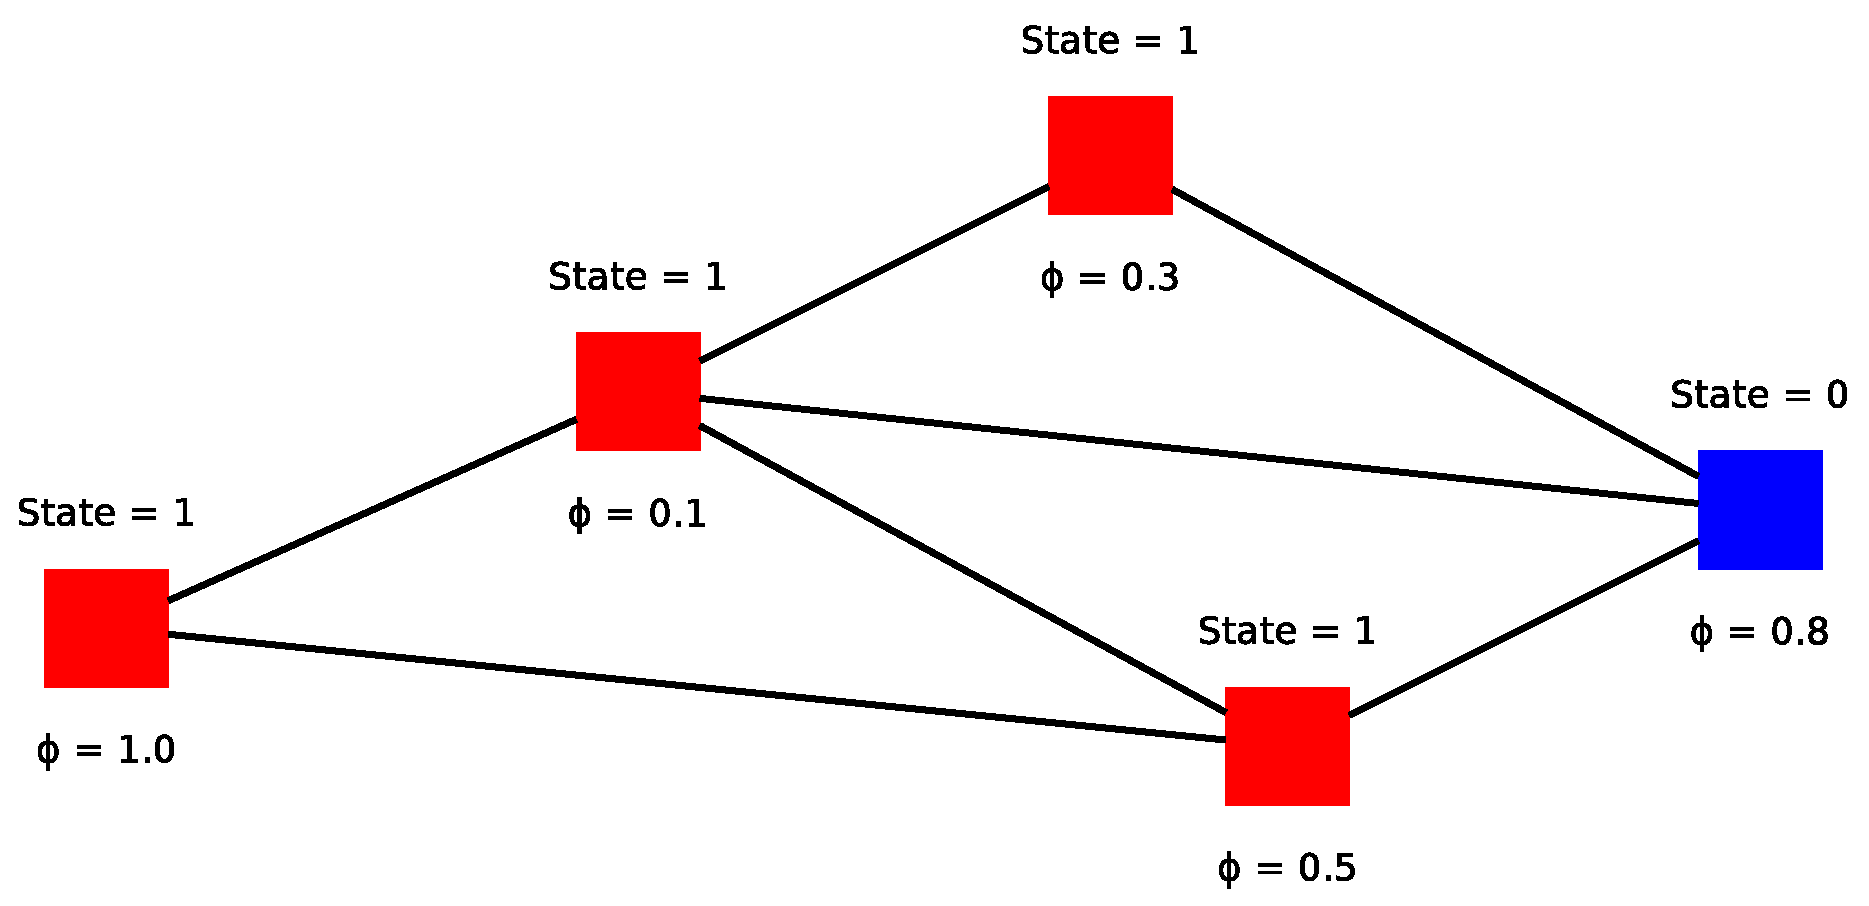
\includegraphics[width=\textwidth]{img/model8}
    \vfill
\end{frame}

\begin{frame}
    \frametitle{Model of Doom}
    \begin{itemize}
        \gitem Coup Successful
    \end{itemize}
    \vspace{8.8pt}
    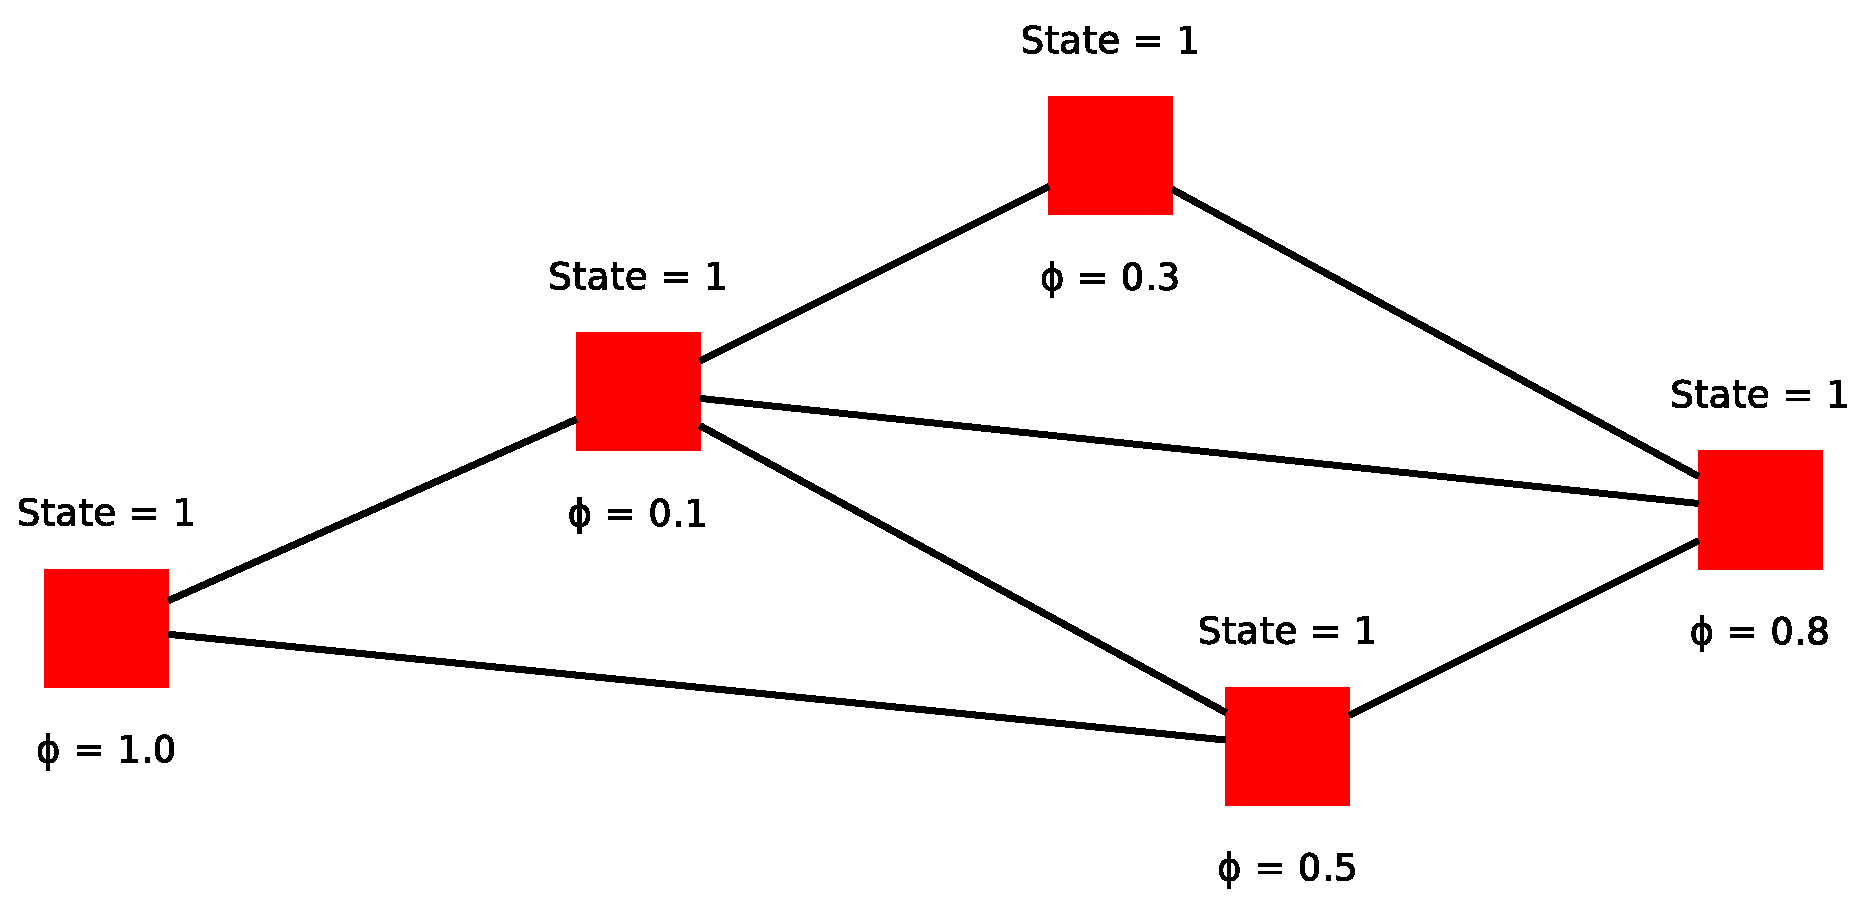
\includegraphics[width=\textwidth]{img/model9}
    \vfill
\end{frame}


\begin{frame}
    \frametitle{Watts' Model}
    \begin{itemize}
        \gitem Each person/agent is a node in a graph
        \gitem Agents have a state $\in \lbrace 0, 1 \rbrace$
        \gitem Agents observe their neighbors
        \gitem Agents change to a state if a fraction of their neighbors has that state
    \end{itemize}
    \vfill
\end{frame}

\begin{frame}
    \frametitle{Watts' Model -- Random Graph}
    \begin{itemize}
        \fitem $n$ nodes
        \fitem $p_k$ propability of $n$ to have $k$ neighbors
        \fitem $z = \left<k\right>$ expectation value or average degree
        \fitem $p_k = \frac{e^{-z}z^k}{k!}$ Poisson-distributed (Erdős–Rényi-Model with $p = \frac{z}{n}$)
    \end{itemize}
    \vfill
\end{frame}

\begin{frame}
    \frametitle{Findings}
    \begin{textblock*}{5cm}(7cm,2.2cm)
        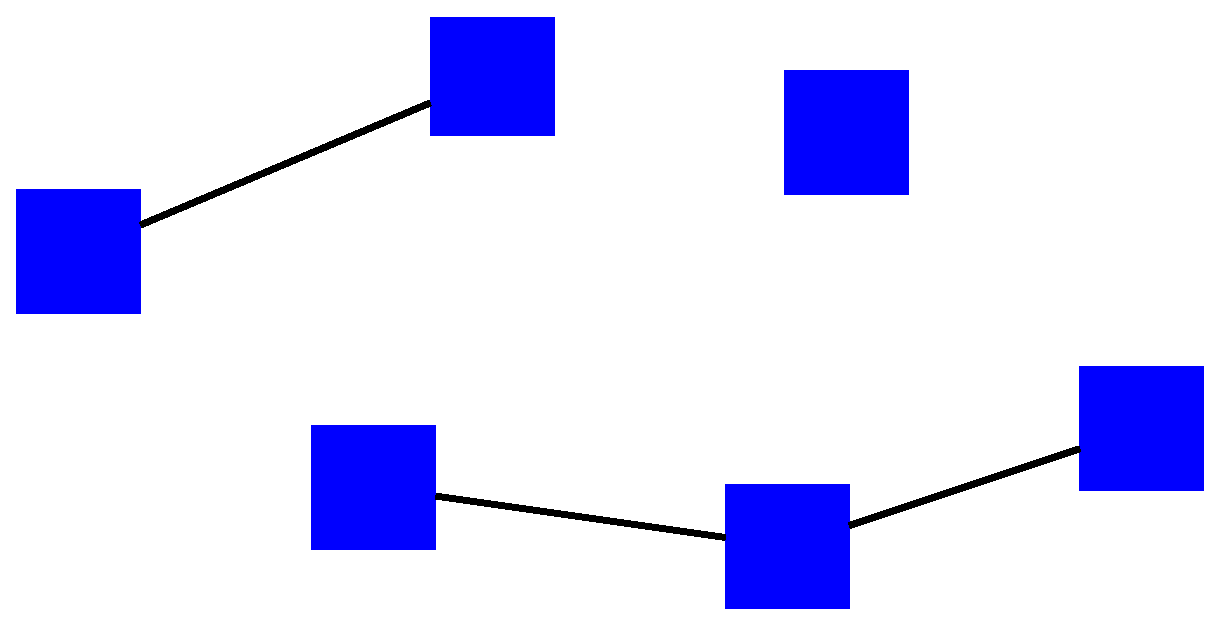
\includegraphics[width=5cm]{img/sparse}
    \end{textblock*}
    \begin{itemize}
        \gitem Cascades in Sparse Networks
        \begin{itemize}
          \fitem Limited by Connectivity
          \fitem Cascade Size Exhibits Power-Law Distribution
          \fitem Most Highly Connected Cluster is Critical Triggers
        \end{itemize}
    \end{itemize}
    \vfill
\end{frame}

\begin{frame}
    \frametitle{Findings}
    \begin{textblock*}{5cm}(7cm,2.2cm)
        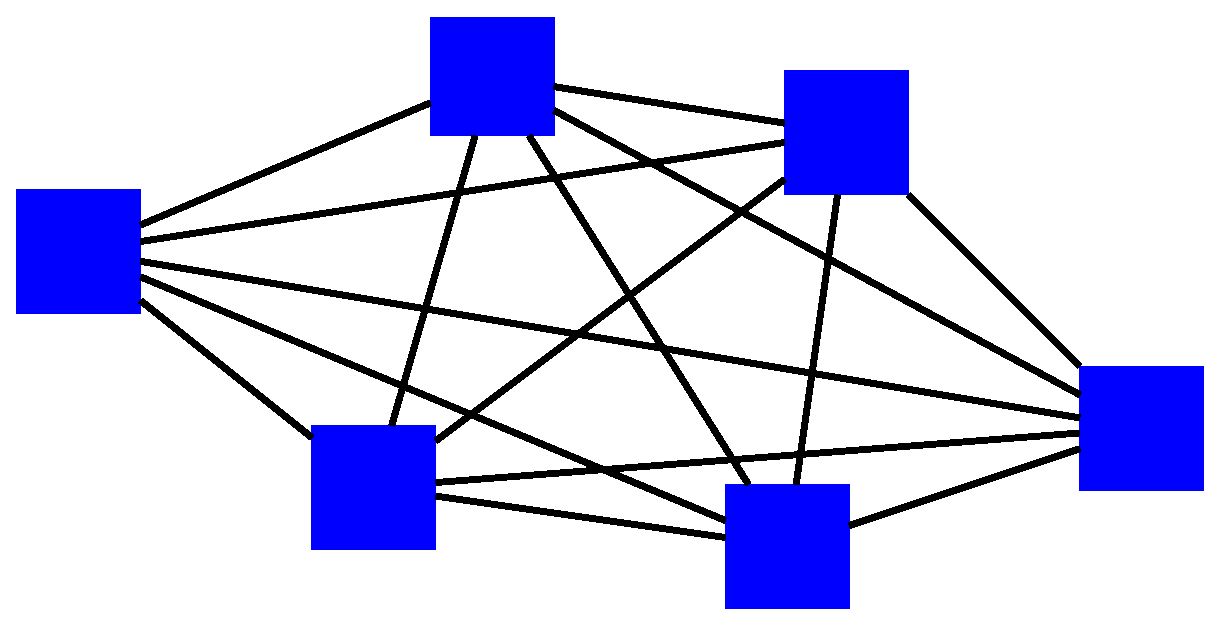
\includegraphics[width=5cm]{img/dense}
    \end{textblock*}
    \begin{itemize}
        \gitem Cascades in Dense Networks
        \begin{itemize}
            \fitem Limited by Threshold
            \fitem Cascade Size Bimodal (Most are Small, Some are Large)
            \fitem Cluster with Average Degrees are Triggers (Because They are Frequent)
        \end{itemize}
    \end{itemize}
    \vfill
\end{frame}

\begin{frame}
  \frametitle{Findings}
  \begin{itemize}
    \fitem Threshold Heterogenity Increases Cascade Likelihood
    \fitem Degree Heterogenity Decreases Cascade Likelihood
  \end{itemize}
  \vfill
\end{frame}

\begin{frame}
    \frametitle{Limitations}
    \begin{itemize}
        \fitem No Personal Knowledge
        \fitem No Global Adoption Rate
        \fitem No Relationship Strength
        \fitem One-Way Threshold
        \fitem Sample Size for Bimodal Distribution Very Limited
        \fitem No Threats to Validity Mentioned
    \end{itemize}
    \vfill
\end{frame}


%%%%%%%%%%%%%%%%%%%%%%%%%%%%%%%%%%%%%%%%%%%%%%%%


\begin{frame}
    \vfill
    \begin{center}
        {\Huge Thank You All For Listening}\
    \end{center}
\end{frame}


\end{document}
